\documentclass[a4paper, 11pt, titlepage]{article}
\usepackage{a4wide}
\usepackage{amsmath}

\usepackage[pdftex]{graphicx}

\usepackage{subcaption}
\usepackage{listings}
\usepackage{color}
\usepackage{cite}
\usepackage{import}


\newcommand{\HRule}{\rule{\linewidth}{0.5mm}}

%Colours!
\usepackage[table]{xcolor}
\definecolor{mygreen}{rgb}{0,0.6,0}
\definecolor{mygray}{rgb}{0.5,0.5,0.5}
\definecolor{mymauve}{rgb}{0.58,0,0.82}
\definecolor{mynavyblue}{HTML}{1E5A9C}

%PDF hyperlinks
\usepackage{hyperref}
\hypersetup{
     colorlinks   = true,
     citecolor    = black,
     linkcolor    = black,
     urlcolor   = mynavyblue,
     bookmarksopen  = false,
     pdfpagemode  = UseNone,
     pdftitle   = {Hexacopter Project 2015 - Ardupilot proposal},
     pdfauthor    = {},
     pdfsubject = {Hexacopter FYP 2015}
}



\begin{document}


  
\begin{titlepage}
\begin{center}

% Upper part of the page. The '~' is needed because \\
% only works if a paragraph has started.

\includegraphics[width=0.7\textwidth]{./logo.png}~\\[1cm]

\textsc{\Large Final Year Project Proposal}\\[0.5cm]

% Title
\HRule \\[0.4cm]
{ \huge \bfseries Towards Autonomous Search and Discovery in UAVs \\[0.4cm] }

\HRule \\[1.5cm]

% Author and supervisor
\noindent
\begin{minipage}[t]{0.4\textwidth}
\begin{flushleft} \large
\emph{Author:}\\
Brett \textsc{Downing}
\end{flushleft}
\end{minipage}%
\begin{minipage}[t]{0.4\textwidth}
\begin{flushright} \large
\emph{Supervisors:} \\
Prof.~Thomas \textsc{Braunl}\\
Chris \textsc{Croft}
\end{flushright}
\end{minipage}

\vfill

% Bottom of the page
{\large \today}

\end{center}
\end{titlepage}

  %\maketitle
  \begin{abstract}
    %what it is, where it fits, what focus do we have
    The low complexity and VTOL capability of multi-rotor Micro-UAVs, and the falling cost of parts lends these platforms to an ever increasing array of autonomous routines from remote inspection to extreme sport chase-cam applications.
    This document outlines a study into using computer-vision to guide navigation routines for object tracking and autonomous remote inspection. 

  \end{abstract}
  \tableofcontents

  \section{Introduction}
    %Buzzword Bingo
    \subsection{Motivation}
    Recent Developments in power and control electronics has allowed small, consumer level UAVs to lift enough processing capacity to navigate at least partly by computer vision.

    A number of Commercial Micro UAVs are beginning to advertise the ability to act as an autonomous chase-cam \cite{Lily} \cite{AirDog}.  Almost all of these systems rely on a tracking device on the user, and many navigate entirely by GPS.  While the performance of GPS is improving, the performance of a chase-cam will be limited to the update rate and fix accuracy of the beacon and drone GPS modules.  It also requires a lock to be achieved in both devices before tracking can commence.

    The power distribution and plant monitoring sectors have recently been taking on small fleets of drones to perform routine inspection of remote, hazardous or otherwise difficult locations \cite{RopeAccess}.  Many of these applications are reasonably repetitive and well defined enough to fully automate, but cannot be navigated by GPS alone due to the poor repeatability of the GPS system. 

    This study will investigate the usability of computer vision alone to track and follow a moving target, and navigate an automated inspection routine of points of interest established by computer-vision.  It is hoped that this work can be used to improve the performance of camera tracking routines in autonomous chase-cam and cinematographic applications, and partially automate remote inspection 

    Much of the technology related to multi-copters is applicable to most other forms of UAV.  The vast array of applications micro UAVs have found suggests this work may find use in Agriculture, mapping, targeted crop dusting, Cinematography, extreme-sport photography, Data collection, remote observation and inspection and hazard and environmental monitoring.


  \subsection{Project History}
  %names, references
    \subsubsection{2013}
    The 2013 team, O'Connor \cite{OConnor} and Venables \cite{Venables} established the project with the purchase of a DJI flame-wheel F550 Hexacopter with a NAZA-lite flight controller.  This copter was fitted and tested, and finally converted into an autonomous platform with the addition of a Raspberry Pi single-board computer (RPi) and a circuit to switch the control channels from the radio receiver to the RPi GPIO outputs.
    The NAZA-lite at this time did not feature telemetry outputs or way-point inputs, but it was able to loiter in a stiff wind using a GPS fix.
    This team gathered location information for the RPi using a Qstarz GPS unit, and bearing information using an X-sens IMU.  The sensor duplication did not exceed the maximum payload capacity of the platform, but it did suffer a short flight-time.
    The drone was able to execute basic way-point navigation.
    \subsubsection{2014}

    The 2014 team, Baxter \cite{Baxter}, Mazur \cite{Mazur} and Targhagh \cite{Targhagh} continued the project adding an internet accessible web UI to control the various autonomous features of the platform, displaying the flight-path of the copter and a live feed of the camera.
    The navigation routines were improved and extended to permit operation without reliable heading information, and the computer vision routines were extented.

    \subsubsection{2015}
    The project is being continued Allen \cite{Allen}, Mohanty \cite{Mohanty}, Tan \cite{Tan} and Downing \cite{Downing}.
    Because of the rapid pace that the market is adopting new features and technologies, we saw fit to undertake a critical review of all aspects of the platform, and begin improvements that facilitate the current typical feature set.

  \section{Literature Review}

  \subsection{Optical Search}
    The UAV Outback Challenge \cite{OutbackChallenge} is a regular competition to perform various search and rescue missions autonomously.  The performance criteria are deliberately set very high, and the competition frequently goes uncompleted.  
    In 2012, CanberraUAV \cite{canberrauav}, a UAV development team from Canberra completed the search aspect of the competition.
    After trying a number of image recognition algorithms, the search algorithm that they flew with simply looked for the blue of the jeans of Outback Joe \cite{tridge}.  This was sufficient to locate the target in a 4x6 km area.

    Multi-copters have received a great deal of attention by merit of their simplicity.  A great deal of design work has come out of hobbyist communities, notably forums 
    such as DIY Drones \cite{DIYDrones} that have been home to 

    \subsection{Altitude Estimation by optical flow}
    \subsection{Optical Navigation IROS}
    \subsection{Chase cam}

    \subsubsection{Notable Technologies}
    Location stabilisation using Optical Flow Odometry
    Altitude estimation using optical flow methods (DIY Drones)
    Aggressive manoeuvres and precision flight with off-board processing
    Machine-Learning Feed-Forward controllers for accurate path following
    Computer Vision searching (Canberra UAV, outback challenge)



    \subsubsection{Existing tools and software}
    Mission Planner:
      Mission Planner is a ground-station program written for UAVs that communicate over the MAVLINK protocol.  There are currently three versions of this software, each built with slightly different compatibilities in mind.  This will probably be our software of choice for monitoring the status of the drone during tests.

    Tower: \cite{3dr-tower}  is an android application that handles most of the features of a ground station on an android phone or tablet.


  \section{Progress Report}
  \subsection{Where we started}
    \subsubsection{Flight Hardware}
      The Hexacopter is a DJI F550 frame with AXI2217 motors and DJI OPTO30A ESCs, 254mm props and a 6Ah 11.1V Lipo battery.
      This platform gives us a generous lifting capacity, and enough flight time to run multiple tests.
      We estimate the power consumption at take-off to be in the region of 50-100A.  A switch had been installed in-line between the battery and the power distribution board. This switch was a 5A rocker switch rated to mains voltage.  Surprisingly, it lasted two full years of testing and only melted shortly after hand-over in 2015.

    \subsubsection{Flight Electronics}
      The 2013 team  decided to use a NAZA-V1-lite flight computer.  This works well for free-flight, but does not make provisions for way-point navigation or telemetry.Interfacing is via Servo signals only, generated by ServoBlaster on the RPi.

      In order to switch between manual and autonomous modes, the 2013 team installed a switching circuit. This circuit featured a 555 timer and four relays.
      There was no schematic, and the only documentation was a copper layout \cite[p. 27-28]{OConnor}.  Only after meeting with the 2014 team did we become aware that there were dead channels on this board due to multiple failed relays.

    \subsubsection{Autonomy Electronics}
      In Autonomous mode, the hexacopter is directed by a Raspberry Pi Model-B Single-Board-Computer.
      This platform is extremely widely used for all manner of projects simply due to its cost.
      It supports Linux and has drivers for almost any hardware we could hope to add to the system. It supports a camera over a dedicated interface.
      The server has a WiFi connection allowing us to remotely control the autonomous features, and even re-configure and recompile components during manual flight.

      The Wireless adapter, the GPS system, and the IMU were all connected via USB, which was powered via the RPi.  The wireless connection would frequently drop out, and the GPS would lose lock or re-connect to USB, causing the navigation routine to lock up.
      The Wiring Harness was undocumented, with links that appeared entirely temporary, but looked as though they had been there for far too long.

    \subsubsection{Autonomy Software}
      The on-board server is currently doing all of the autonomous navigation processing.  This works reasonably well for slow manoeuvres but the latency in data collection, and the generation and re-interpretation of control signals leaves the Pi at a distinct performance disadvantage to autonomous routines running on the flight-computer.

      The Pi runs a basic webserver hosting a page with basic autonomy controls. We can engage various

    \subsubsection{Sensors and auxiliary Hardware}
      The camera is stabilised for pitch and roll by two servos. The tilt servo was damaged and tilt stabilisation was almost non-existent.  The servos receive correction information from the flight computer with a configurable gain parameter.  The servos are able to hold the camera level in the steady state, but have a significantly delayed response.

      The server collected position data from a second GPS module (QStarz).  This GPS module appears to have a filtering scheme with dead-reckoning configured for automotive applications; It exhibited lazy vertical response, and low accelerations.

      Bearing data was to be collected from an X-sens branded IMU, though this was not installed at the time of hand-over, possibly due to an unreasonably heavy wiring harness.  Instead, the navigation loops in the old code-base estimated the bearing by flying forward for a fixed interval before beginning navigation, relying on the flight computer to hold the bearing for the duration of the mission.

  \subsection{What we've achieved}

    \subsubsection{Flight Electronics}
      With the drop-outs in wireless and GPS very nearly causing a crash, We ran a full tear-down of the copter's electronics and uncovered quite a serious power supply contention issue; the NAZA's power supply was connected via the relay board to the RPi which was supposed to be powered by a different power module (a potted 5V regulator).  Correcting the contention problem and repairing damaged links, the reliability of the copter was improved, but our faith was shaken.  
      We reverse-engineered the switching circuit installed by the 2013 group, and traced the wiring harness into a net-list.  Having talked to the previous teams, we appear to have generated better documentation about the hardware than the teams had worked with initially.
      \begin{figure}[h!]
        \centering
        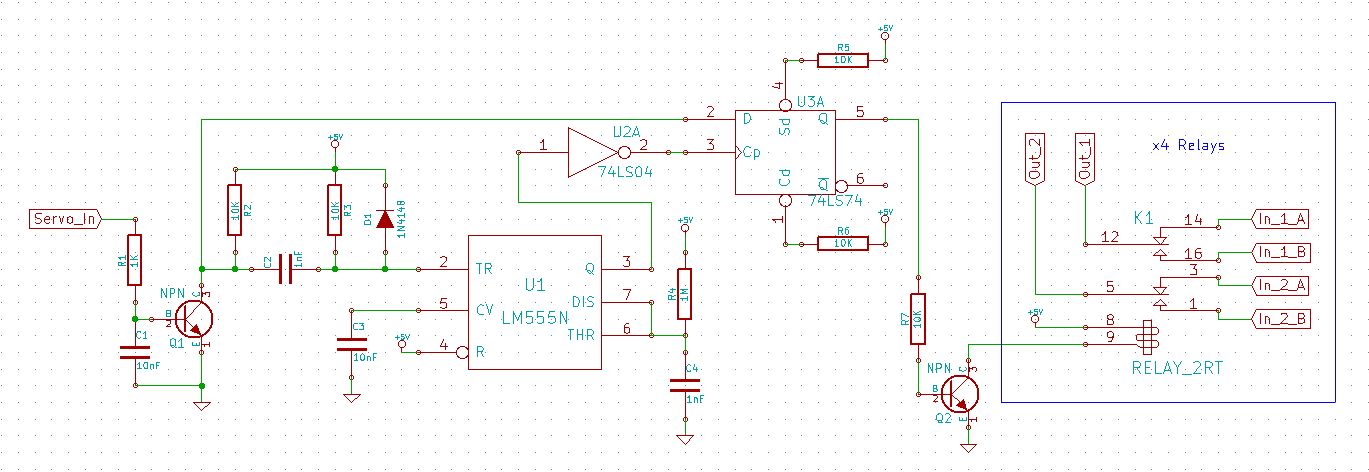
\includegraphics[width=0.8\textwidth]{SwitchCircuit.png}
        \caption{The circuit used to switch between the pilot and the autopilot}
      \end{figure}
      The power switch was replaced with a 15A toggle switch, still woefully under-rated, and mounted inconveniently close to the props.  It was finally removed in favour of isolating the battery at the connector which was easier to get to anyway.


    \subsubsection{Landing Gear}
      We were encouraged to learn to pilot the copter, flying it on a regular basis.  Naturally, the copter was crashed a couple of times, and was damaged in almost every instance.  We inspected the damage and considered options to make the drone more tolerant to heavy landings, or at least make the crashes slightly cheaper.
      We removed the MDF arm extensions which appeared to be coupling the energy of the crash into torque on the arms, and installed long injection-moulded legs that flex a long way. This gives us more room underneath the copter for future enhancements, increases the total survivable impact energy, and should help to limit crash damage to single, cheap components that can be replaced easily.

    \subsubsection{Failsafe Recovery}
      At hand-over the copter was meant to implement a return-to-launch fail-safe in the event of transmitter failure.  We found the fail-safe configurations empty on both the controller and the NAZA, and corrected this omission.

    \subsubsection{Software}
      The code-base of the previous year-groups did not appear to use version-control consistently, or at all in some cases.  Many of the function files were duplicated, and functionality was not modularised.
      With the heroic efforts of Tan \cite{Tan}, we've implemented and tested a great deal of code that we were able to salvage from the previous year-groups.  
      Oddly, our tests of the previous year-groups' code have produced better results than are published in the respective papers.  However the claims of the previous groups still appear grossly overstated.

      The object tracking code we ported over from the 2014 team took a relatively simplistic approach, feeding the pixel position from the image directly into two PID controllers.  This did work, but altitude, camera angle, parallax, and other variables tended to make the controller go from a-bit-weak, to utterly unstable with what seemed like minor environmental changes.

      We've built up the code-base to estimate the physical position of the target in coordinates relative to the copter, trying to sanitize the inputs to the control loop. The control loop now takes inputs of the target's physical coordinates in metres.  Our controller is still a collection of basic PID loops, but already, the behaviour is far more consistent in flight.

    \subsubsection{Major Upgrades}
      We've made a proposal and ordered parts to remove the NAZA-V1-Lite flight computer and replace it with a 3D-Robotics Pixhawk \cite{3dr-pixhawk} running the Ardupilot flight control software.  (as of submission of this paper, work will be under way to install and test the Pixhawk.)
      This change allows us to utilise the vast array of supporting software that the Ardpilot community has written including ground-stations, telemetry loggers, Smart-phone apps, Kalman navigation filters and automatic flight control tuning.  It also exposes all of the live flight parameters, raw and processed, available over a documented interface.  This decision was partly motivated by our observations of an older APM-2.6 flight computer running similar firmware.

    \subsubsection{Autonomy Electronics}
      With the limited processing power of the RPi model B, the computer-vision routines were quite sluggish, we have upgraded to the Raspberry Pi Version 2 which has a higher core speed, multiple cores, and more advanced processor optimisations.

      The mass of sensor duplication was a major contributing factor in the short flight-time of the platform.  The NAZA already has GPS and IMU data, sharing it with the RPi seemed like an obvious solution.  The X-sens IMU was only being used for bearing data, and the NAZA's GPS stand contained its compass.
      We found a forum that had a reverse-engineering effort for this protocol\cite{NAZArev}, and ported it to the Pi and its hardware serial port.  This connection gives us access to the same GPS data that the flight computer is working with, reducing controller conflicts. It also gives us access to the NAZA's raw magnetometer data which could be used for bearing, but the inherent biases and changes due to unknown pitch and roll make this data difficult to use.
      The NAZA GPS system uses a basic TTL-level serial protocol, but the message payloads are XORed with an obscure bit combination from the payload itself.  It looks as though the protocol was deliberately obfuscated by DJI.
      After breaking into the NAZA GPS, and in preparation to change to the Pixhawk, the X-sens IMU was never added to the copter and the drivers were removed from the code-base, and we permanently removed Q-starz GPS module.
      

  \subsection{Aims}

    \subsubsection{Hardware Modifications}
      Following the critical review of the hexacopter hardware, we intend to continue development to bring the platform to a respectable standard. These changes started with corrections to the wiring harness, replacement of the landing gear and will continue with the change to the Pixhawk flight computer as discussed in Appendix !!!.
      The servo driven camera gimbal is showing limitations in its abilty to stabilise the camera, but more testing is required before we can make an honest evaluation of its performance and recommend changes.
      A large number of the algorithms we have discussed to identify or track objects require slightly more information than is readily available from the camera alone.  A variety of additional algorithms and sensors will be investigated during the course of this project to fill these information gaps.

    \subsubsection{Go Fetch}
      The focus of this project is to position the UAV based largely on information from the camera.  We intend to continue the development of the object tracking code initially by improving the copter's ability to follow a highly visible target.  This will allow us to perform reasonably aggressive manoeuvres under computer-vision guidance that should highlight weaknesses in the existing software chain.
    %chase and inspect a moving train
    %position estimation

    \subsubsection{Lost and Found}
    \label{sec:Lost and Found}
      The copter is already beginning to exhibit strong tracking behaviour, but we have encountered a camera stability issue (Discussed in \ref{sec:Camera Stability}).
      We've not yet been able to apply aggressive parameters to the chase algorithm because of the instabilities it introduces, and the tracked object frequently leaves the field of view of the camera at the extremes of the controller oscillations.
      We intend to write a search algorithm to attempt to locate an object shortly after it has left the frame, and address the camera stability problem.
      %We intend to write a series of algorithms to construct a weighted search-space based on the previous motion of the target.  This extrapolation will require some kind of prediction engine incorporating known properties of the target's possible motion. 

    \subsubsection{Everything in Its Place}      
    %   to assess the stability of the positioning loop, and the stability of the target estimation algorithm.
     % Object Tracking, chase-cam, remote positioning.

      We expect to improve on the physicality of our control systems, estimating latitude and longitude of the target to assist in lost-target recovery (Section \ref{sec:Lost and Found}).  Logging the estimates of the target's global coordinates is likely to lead to insights into the stability and validity of our work, and suggest possible improvements.

      We'd like to convert the loop to calculate the desired location of the drone based on the location of the targets that have been spotted, regardless of which objects are currently in the frame.  This would provide a foundation for a Simultaneous Localisation and Mapping (SLAM) system.

      Ideally, we'd use this information to calculate appropriate observation locations as way-points for remote inspection, and construct no-fly-zones around visible obstructions.  Getting this far will rely heavily on tightly integrating work from all members of the team, and may not be feasible in light of our time constraints.

  \subsection{Major Challenges}
    \subsubsection{Limiting Controller Complexity}
      A method for the copter to chase an object on a screen is a relatively straight-forward problem to grasp intuitively, but include camera geometry, position estimation, velocity and acceleration limits and such; just defining the problem rapidly turns into a wall of mathematics.  We've made a lot of progress towards sensible estimation and chase routines already, but already the single-input-single-output PID controllers are becoming inadequate. The control scheme will need to be analysed in a more comprehensive manner, incorporating data sets from multiple sources to coordinate coherent actions in a multi-input-multi-output controller.

      Limiting the scope and complexity of the controller may well become a matter of identifying diminishing returns.  Rigorous flight performance analysis using sensible metrics, monitoring the time spent coding those incremental improvements, and assessing the wider applicability of the possible changes may help to identify when the chase controller should be declared "good enough".


    \subsubsection{Flying on a Steady Cam}
    \label{sec:Camera Stability}
      As the platform stands, the camera gimbal does not sufficiently isolate platform motion to stabilise a simple control loop.
      For example, a forward motion instruction from the chase algorithm causes the copter's rear rotors to throttle up, then the platform pitches forward, then the copter accelerates forward.  The pitch data from the IMU is sent to the camera stabilisation servo which has a slow slew rate and a small delay time.  This delay couples pitch motion into the image processing loop and adds a brief but intense upward swing to the location of the target in the image as the copter accelerates.
      This behaviour is controlled by the physical properties of the copter, the flight-computer's control loops, the servo's controller and the shutter lag on the camera.
      While all of this is technically possible to compensate for, calibrating against mechanical and electrical properties of a commodity servo and an advanced flight controller introduces a large number of variables and doesn't lend itself easily to empirical validation.  

      It makes more sense to solve single whole problems; either cleanly stabilising the camera with a higher performance gimbal, or applying software image stabilisation using motion data from the flight controller to calculate through bulk motions, followed by optical flow methods to remove the remaining jitter.
      The change to the Ardupilot flight computer will give us access to IMU data required for software stabilisation, but it may prove too computationally intensive for the RPiV2 to process.  Many of the parts involved in image stabilisaiton were not selected with any great care, and we fully expect to continue swap out or modify older parts of the copter during the course of the project.

    \subsubsection{Reliability and Repeatability}
    \label{sec:Reliability}
      %When we were first shown the platform, my first thoughts were WTF is all that spaghetti doing on a flying machine.
      Between dead servos, incomplete configurations, undocumented custom circuits with supposedly known but undocumented faults, and a wiring loom that was unreliable, undocumented, and even simply incorrect;  we've been set back by days at a time with intermittent faults.
      Maintaining a high quality of work over a long project is difficult; small, temporary hacks tend to become permanent fixtures and intermittent faults are left undiagnosed with time being prioritised to flashy achievements.

      The change to the Pixhawk is set to remove, modify, and simplify a large portion of the wiring harness.  This is probably the best opportunity to do clean-room engineering on the hardware.  We believe we have the technical skill in the group to leave the wiring harness at least presentable, if not bullet-proof.
      Though it may become necessary to dedicate significant blocks of time to removing temporary fixtures periodically throughout the course of the project.

    \subsubsection{Extensible Code}
      As with incremental hardware modifications, maintaining a high degree of quality across the board is difficult.  
      For this to happen, our code needs to reasonably well documented, modular, conform to some kind of standard, and be logged in version control. 
      Our team has selected projects that are able to begin very independently and achieve clearly defined goals, but as these new capabilities mature, they will be used to enhance aspects of the projects of other team members.  We hope that this cross-project extensibility measure will force some level of accountability to documentation and code cleanliness.



  \section{References}
    Holographic transforms
    Target coordinate estimation with landmarks
    Optical flow uncertainty map
    Altitude estimation using optical flow methods

%Referencing
%---------------------------------------------------------
%\pagebreak
\renewcommand{\refname}{References}
\addcontentsline{toc}{part}{References}
\bibliography{references/refs}
\bibliographystyle{ieeetr}
%\addbibresource{references/refs.bib}
%\printbibliography

%---------------------------------------------------------






	
\end{document}

